\section{Automated Evaluation and Judge Models}

\begin{frame}{}
    \LARGE Research Frontiers: \textbf{Judges Under Pressure}

    \vspace{1em}
    \normalsize What happens to a judge once we train it, and then train against it?
\end{frame}

\begin{frame}{From Prompted Judges to Trained Judges}
    \begin{itemize}\itemsep0.35em
        \item The evaluation deck covered judge prompts, biases and calibration against humans. Since then, judges became \textbf{trained models}, and their scores became \textbf{rewards}.
    \end{itemize}
    \begin{center}
    \small
    \renewcommand{\arraystretch}{1.12}
    \begin{adjustbox}{max width=\linewidth}\begin{tabular}{llc}
        \toprule
        \textbf{Judge} & \textbf{How it was validated} & \textbf{Result} \\
        \midrule
        Prometheus (13B, 2023) & Pearson with human scores & 0.897 (GPT-4: 0.882) \\
        JudgeLM (7B, 2023) & agreement with its GPT-4 teacher & over 90\% \\
        \midrule
        \multicolumn{3}{l}{\textbf{JudgeBench (2025): pick the objectively correct answer of two. Chance is 50\%.}} \\
        \midrule
        Prometheus 2 (8x7B) & & \alert{40.29\%} \\
        GPT-4o & & 56.57\% \\
        \rowcolor{KAUSTcyan!12} o1-preview & & 75.43\% \\
        \bottomrule
    \end{tabular}\end{adjustbox}
    \end{center}
    \begin{itemize}\itemsep0.35em
        \item \textbf{``Agrees with GPT-4'' is not ``is right''.} Fine-tuned judges win in their own domain and generalise worse. In practice they are task-specific classifiers.
    \end{itemize}
    \src{Kim et al., ``Prometheus,'' \href{https://arxiv.org/abs/2310.08491}{arXiv:2310.08491}. Zhu, Wang, Wang, ``JudgeLM,'' \href{https://arxiv.org/abs/2310.17631}{arXiv:2310.17631}. Tan et al., ``JudgeBench,'' ICLR 2025, \href{https://arxiv.org/abs/2410.12784}{arXiv:2410.12784}. Huang et al., \href{https://arxiv.org/abs/2403.02839}{arXiv:2403.02839}.}
\end{frame}

\begin{frame}{Reward Models as Evaluators: Which Benchmark Predicts RLHF?}
    \begin{columns}[T,onlytextwidth]
        \column{0.36\textwidth}
        \centering
        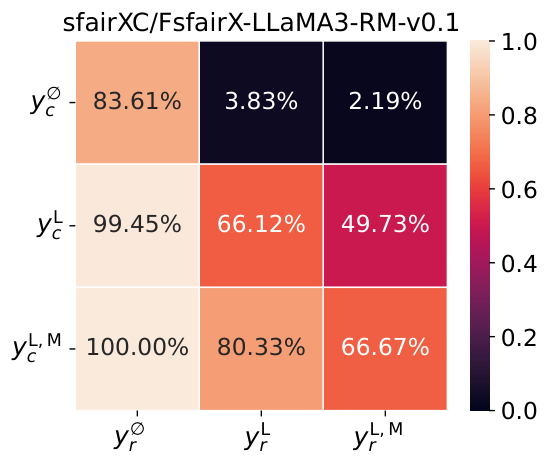
\includegraphics[width=\linewidth,height=0.46\textheight,keepaspectratio]{images/research-frontiers/rmbench_fig2_style_substance_matrix.png}

        {\scriptsize RM-Bench accuracy by style of the chosen (rows) and rejected (columns) answer. Upper right: the correct answer is plain, the wrong one is polished.}
        \column{0.62\textwidth}
        \begin{itemize}\itemsep0.4em
            \item A reward model is a judge whose score is optimised (Day 3). Its benchmark should predict the \emph{policy}.
            \item \textbf{RewardBench saturated.} Among top models its score correlates \emph{negatively} with downstream RLHF quality.
            \item \textbf{Style leaks into preference.} On RM-Bench the best model averages 70.1, and \alert{46.6} on the hard cells. Below chance.
            \item \textbf{RewardBench 2:} unseen human prompts, best-of-4, about 20 points harder. Pearson 0.87 with best-of-$N$ sampling quality.
            \item \textbf{No universal ranking.} In PPO, a reward model from a different base lineage than the policy does markedly worse.
        \end{itemize}
    \end{columns}
    \vspace{0.2em}
    \src{Liu et al., ``RM-Bench,'' \href{https://arxiv.org/abs/2410.16184}{arXiv:2410.16184}, Figure 2 and Table 3. Frick et al., \href{https://arxiv.org/abs/2410.14872}{arXiv:2410.14872}. Lambert et al., ``RewardBench,'' \href{https://arxiv.org/abs/2403.13787}{arXiv:2403.13787}. Malik et al., ``RewardBench 2,'' \href{https://arxiv.org/abs/2506.01937}{arXiv:2506.01937}.}
\end{frame}

\begin{frame}{Generative Verifiers: Judges That Think Before They Score}
    \begin{columns}[T,onlytextwidth]
        \column{0.55\textwidth}
        \begin{itemize}\itemsep0.4em
            \item A scalar reward head cannot reason. A \textbf{generative} reward model writes a critique, then a score.
            \item \textbf{DeepSeek-GRM} first writes the \emph{principles} $p$ to judge by, then the critique $\mathcal{C}$, then extracts scores:
            \[
                p \sim p_\theta(x, y), \quad \mathcal{C} \sim r_\theta(x, y, p), \quad S = f_{\text{extract}}(\mathcal{C})
            \]
            \item The verdict is sampled, so \textbf{judging scales with inference compute}: sample $k$ times and vote, or let a meta reward model filter.
            \item Accuracy: 69.9 with one sample, 72.8 with 32. GPT-4o as a judge: 71.3.
        \end{itemize}
        \column{0.43\textwidth}
        \centering
        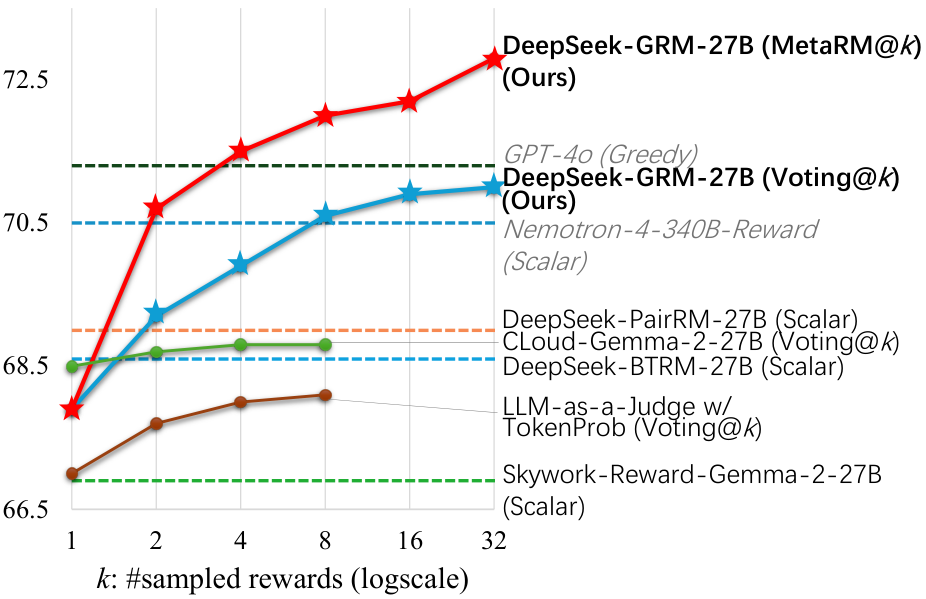
\includegraphics[width=\linewidth,height=0.56\textheight,keepaspectratio]{images/research-frontiers/deepseek_grm_fig1_inference_scaling.png}
    \end{columns}
    \vspace{0.2em}
    \src{Liu et al., ``Inference-Time Scaling for Generalist Reward Modeling'' (DeepSeek), \href{https://arxiv.org/abs/2504.02495}{arXiv:2504.02495}, Figure 1 and Table 2. Zhang et al., ``Generative Verifiers,'' ICLR 2025, \href{https://arxiv.org/abs/2408.15240}{arXiv:2408.15240}.}
\end{frame}

\begin{frame}{Rubrics: Making Open-Ended Answers Checkable}
    \begin{columns}[T,onlytextwidth]
        \column{0.56\textwidth}
        \begin{itemize}\itemsep0.45em
            \item \textbf{HealthBench:} 5,000 conversations and 48,562 criteria written by 262 physicians, each worth $-10$ to $+10$ points. The score is points earned over the maximum, clipped to $[0,1]$.
            \item Scores: GPT-3.5 Turbo 0.16, GPT-4o 0.32, o3 0.60.
            \item \textbf{Rubrics as rewards:} use the rubric score as the RL reward. Up to 31\% relative gain over a plain Likert-score reward.
            \item \textbf{And then Goodhart.} The training judge's score keeps rising while a gold judge's score peaks and falls. Remedy: hide 30 to 50\% of the criteria at each step.
        \end{itemize}
        \column{0.42\textwidth}
        \centering
        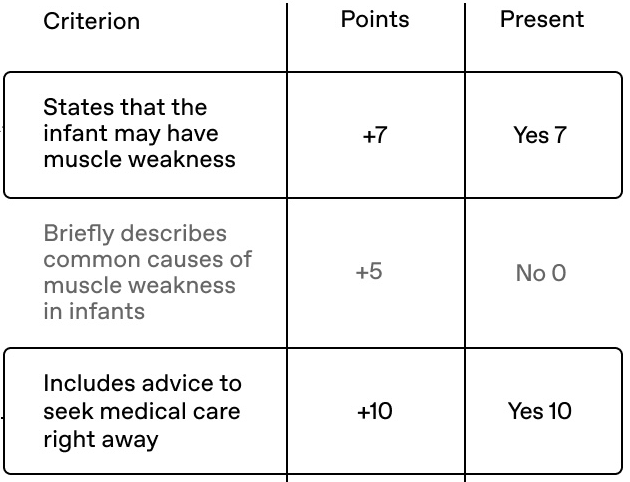
\includegraphics[width=\linewidth,height=0.6\textheight,keepaspectratio]{images/research-frontiers/healthbench_infographic_rubric.png}

        {\scriptsize Part of a HealthBench rubric for one response.}
    \end{columns}
    \vspace{0.2em}
    \src{Arora et al., ``HealthBench'' (OpenAI), \href{https://arxiv.org/abs/2505.08775}{arXiv:2505.08775}, infographic (cropped). Gunjal et al., ``Rubrics as Rewards'' (Scale AI), \href{https://arxiv.org/abs/2507.17746}{arXiv:2507.17746}. Yang et al., ``Rubric Dropout,'' \href{https://arxiv.org/abs/2608.11669}{arXiv:2608.11669}.}
\end{frame}

\begin{frame}{Attacking the Judge: One Token Is Enough}
    \centering
    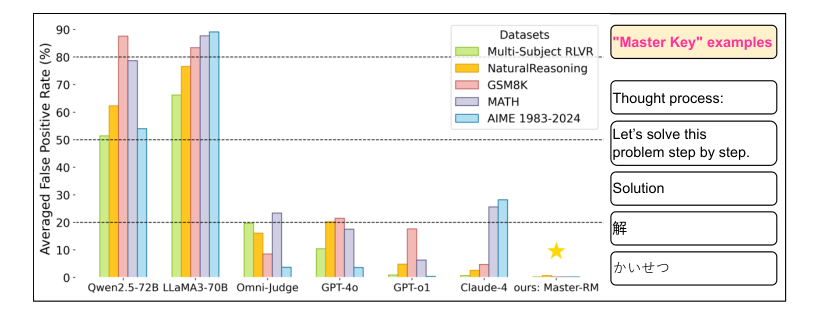
\includegraphics[width=0.9\linewidth,height=0.42\textheight,keepaspectratio]{images/research-frontiers/onetoken_fig1_rlvr_collapse.png}
    \begin{itemize}\itemsep0.35em
        \item \textbf{How it was found.} An RL policy trained against an LLM judge collapsed to answers such as ``Solution''. The judge kept marking them correct.
        \item \textbf{Master keys:} a space, a colon, ``Thought process:''. GPT-4o's false-positive rate reaches 35\% on punctuation and 60 to 90\% on ``Thought process:''.
        \item \textbf{Fix:} train the judge on 20K adversarial negatives. False positives fall to about zero.
    \end{itemize}
    \src{Zhao et al., ``One Token to Fool LLM-as-a-Judge'' (Princeton, Tencent), \href{https://arxiv.org/abs/2507.08794}{arXiv:2507.08794}, Figure 1 and Table 1.}
\end{frame}

\begin{frame}{Judging Agents, and Judging the Leaderboards}
    \begin{itemize}\itemsep0.4em
        \item \textbf{Agent-as-a-Judge (Meta and KAUST).} Give the judge tools to open files and check requirements. It agrees with human consensus about 90\% of the time, against 60 to 84\% for an LLM judge, at \$30.58 against \$1,297.50 for human graders.
        \item \textbf{The Leaderboard Illusion (2025).} One provider tested 27 private variants before a launch and published the best. Identical checkpoints scored 17 points apart.
        \item \textbf{Arena AutoEval (July 2026).} A reward model trained on millions of votes now scores new models on day one. Models within 5 points cannot be told apart.
    \end{itemize}
    \src{Zhuge et al., ``Agent-as-a-Judge,'' \href{https://arxiv.org/abs/2410.10934}{arXiv:2410.10934}. Singh, Nan, Wang et al., ``The Leaderboard Illusion,'' \href{https://arxiv.org/abs/2504.20879}{arXiv:2504.20879}. Arena Team, ``Our Response to `The Leaderboard Illusion'\,'' (2025) and ``Introducing AutoEval'' (2026).}
\end{frame}

\begin{frame}{Judges: What to Remember}
    \begin{itemize}\itemsep0.55em
        \item Judges are now \textbf{trained reward models}. Validate them on \emph{objective correctness}, not on agreement with a teacher.
        \item A reward-model benchmark matters only if it \textbf{predicts the downstream policy}.
        \item \textbf{Generative verifiers} turn judging into reasoning, and scale with inference compute.
        \item \textbf{Rubrics} make open tasks checkable, and are hacked as soon as they are optimised.
        \item Judges have \textbf{attack surfaces}. Leaderboards have \textbf{incentives}.
    \end{itemize}
    \vspace{0.4em}
    \takeaway{\textbf{Next.} With these instruments and their limits in mind, we can read the scoreboard. What do the frontier models of October 2026 look like, and who is ahead?}
\end{frame}
